
%
% foundations - clustering algorithms
%

\section{Clustering algorithms}

Researchers have created a multitude of algorithms, each appropriate for a certain task. As we will find out later, the requirements to the spatial clustering algorithm for this thesis are specific, which out-rules most scientific clustering algorithms which are geared towards image recognition or other disciplines. To provide an overview and to understand the basic differentiation of clustering techniques explained in \ref{chapter:clustering-techniques}, in this chapter we will introduce 4 foundational clustering algorithms:

\begin{itemize}
\item {K-means (Squared Error Algorithm)}
\item {Agglomerative Hierarchical Clustering Algorithm}
\item {DBSCAN (Density-based)}
\item {STING (Grid-based)}
\end{itemize}

\subsection{Squared Error Algorithms: K-means}
\label{chapter:k-means}

The K-means is the most commonly used and simple algorithm based on a \textit{squared error criterion}. It creates a one-level partitioning of the data items by dividing them into \textit{K} clusters. By starting with a random initial partition, it iteratively reassigns the patterns to clusters based on similarity.  The clustering process is completed when a convergence criterion is met, i.e. no further reassignments happen. Clusters are defined by \textit{cluster prototypes}: the centroid of the clustered items. Alternatively, the \textit{K-medoid} algorithm uses the most representative data item instead of the centroid.

The time complexity of the K-means algorithm is linear to the number of points:
\[time~complexity = \BigO{n}\]

\begin{algorithm}[t]
  \SetKwInOut{Input}{input}
  \Input{the number of clusters, $K$}
  \BlankLine
  {Select $K$ points as initial centroids}\;
  \While{Centroids do change}{
    {Form $K$ clusters by assigning each point to its closest centroid}\;
    {Recompute the centroid of each cluster}\;
  }
  \caption{K-means algorithm~\cite{Meert06clustermaps}}
  \label{alg:k-means}
\end{algorithm}

The selection of initial centroids affects the final outcome of the clustering process. Choosing them randomly is a simple, but not very affective approach. This can be compensated by applying multiple runs of the algorithm, to retrieve an optimal result set. Optimizations to the centroid initialization include applying a hierarchical clustering or selecting distant points in the beginning.

Assigning points to the closest centroid requires a proximity measure, as explained in \ref{chapter:proximity}. Simple measures like the Euclidian distance are preferred, as this step needs to happen repeatedly within the algorithm. For each cluster, the centroid needs to be recalculated afterwards. This procedure is repeated until centroids do not change any more \cite{Jain99clusterreview, Meert06clustermaps}.

Figure \ref{fig:clustering_k-means} illustrates a K-means clustering process.

\begin{figure}[h]
  \begin{center}
    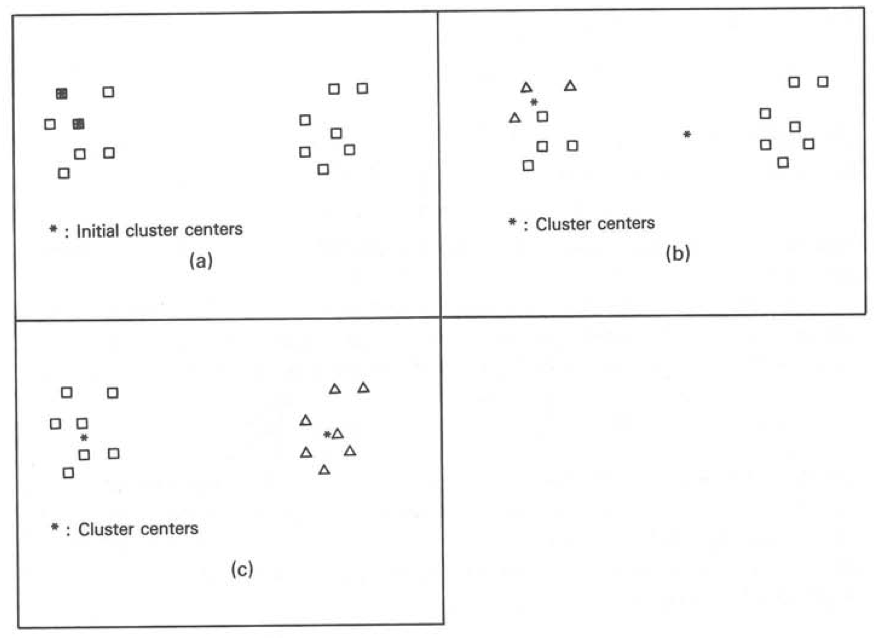
\includegraphics[width=1\textwidth]{figures/clustering_k-means.png}
    \caption{Convergence of K-means clustering: (a) initial data; (b) cluster membership after first loop; (c) cluster membership after second loop~\cite[p 99]{Jain88clustering}.}
    \label{fig:clustering_k-means}
  \end{center}
\end{figure}


\subsection{Agglomerative Hierarchical Clustering Algorithm}
\label{chapter:clustering-hierarchical}

This exemplary, \textit{hierarchical clustering algorithm} creates a hierarchy of nested sub clusters by serial partitioning. Its \textit{agglomerative} nature makes it start with every data item as a single cluster and merge them sub-sequentially. As an alternative, a \textit{divisive} hierarchical clustering would start with one cluster containing all data points and recursively split them up. At each level, a partitioning can be extracted, for example to serve as initial set of centroids for the previously discussed K-means algorithm. 

The time complexity of the agglomerative hierarchical clustering algorithm is:
\[time~complexity = \BigO{n^3}\]

\begin{algorithm}[t]
  {Assign each point to its individual cluster}\;
  {Compute the proximity matrix}\;
  \While{Number of clusters is larger than one}{
    {Merge the closest two clusters}\;
    {Update the proximity matrix to reflect the proximity between the new cluster and the original clusters}\;
  }
  \caption{Agglomerative hierarchic algorithm~\cite{Meert06clustermaps}}
  \label{alg:hierarchical}
\end{algorithm}

At the beginning of the agglomerative hierarchical clustering algorithm, each point is assigned to its own cluster. A proximity matrix is calculated to store the distances for all pairs of data items based on the chosen proximity measure.

To merge the two closest clusters, different heuristics may be applied. Most importantly, \textit{single-link} hierarchical clustering algorithms measure the distance between two clusters by the \textit{minimum} distance between all pairs of items from the two clusters. In contrast, \textit{complete-link} algorithms use the \textit{maximum} distance to create compact clusters and prevent chaining effects. Other approaches are based on \textit{average linkage} or \textit{Ward's method}. After merging the clusters, the proximity matrix will be updated, so that it reflects the current state of the clustering process. This procedure is repeated until all clusters have been merged, each step in the loop yields a level in the hierarchical clustering~\cite{Jain88clustering, Jain99clusterreview, Meert06clustermaps}.

Figure~\ref{fig:clustering-hierarchical-dendrogram} illustrates a Agglomerative Hierarchical clustering process as a dendrogram.

\begin{figure}[h]
  \begin{center}
    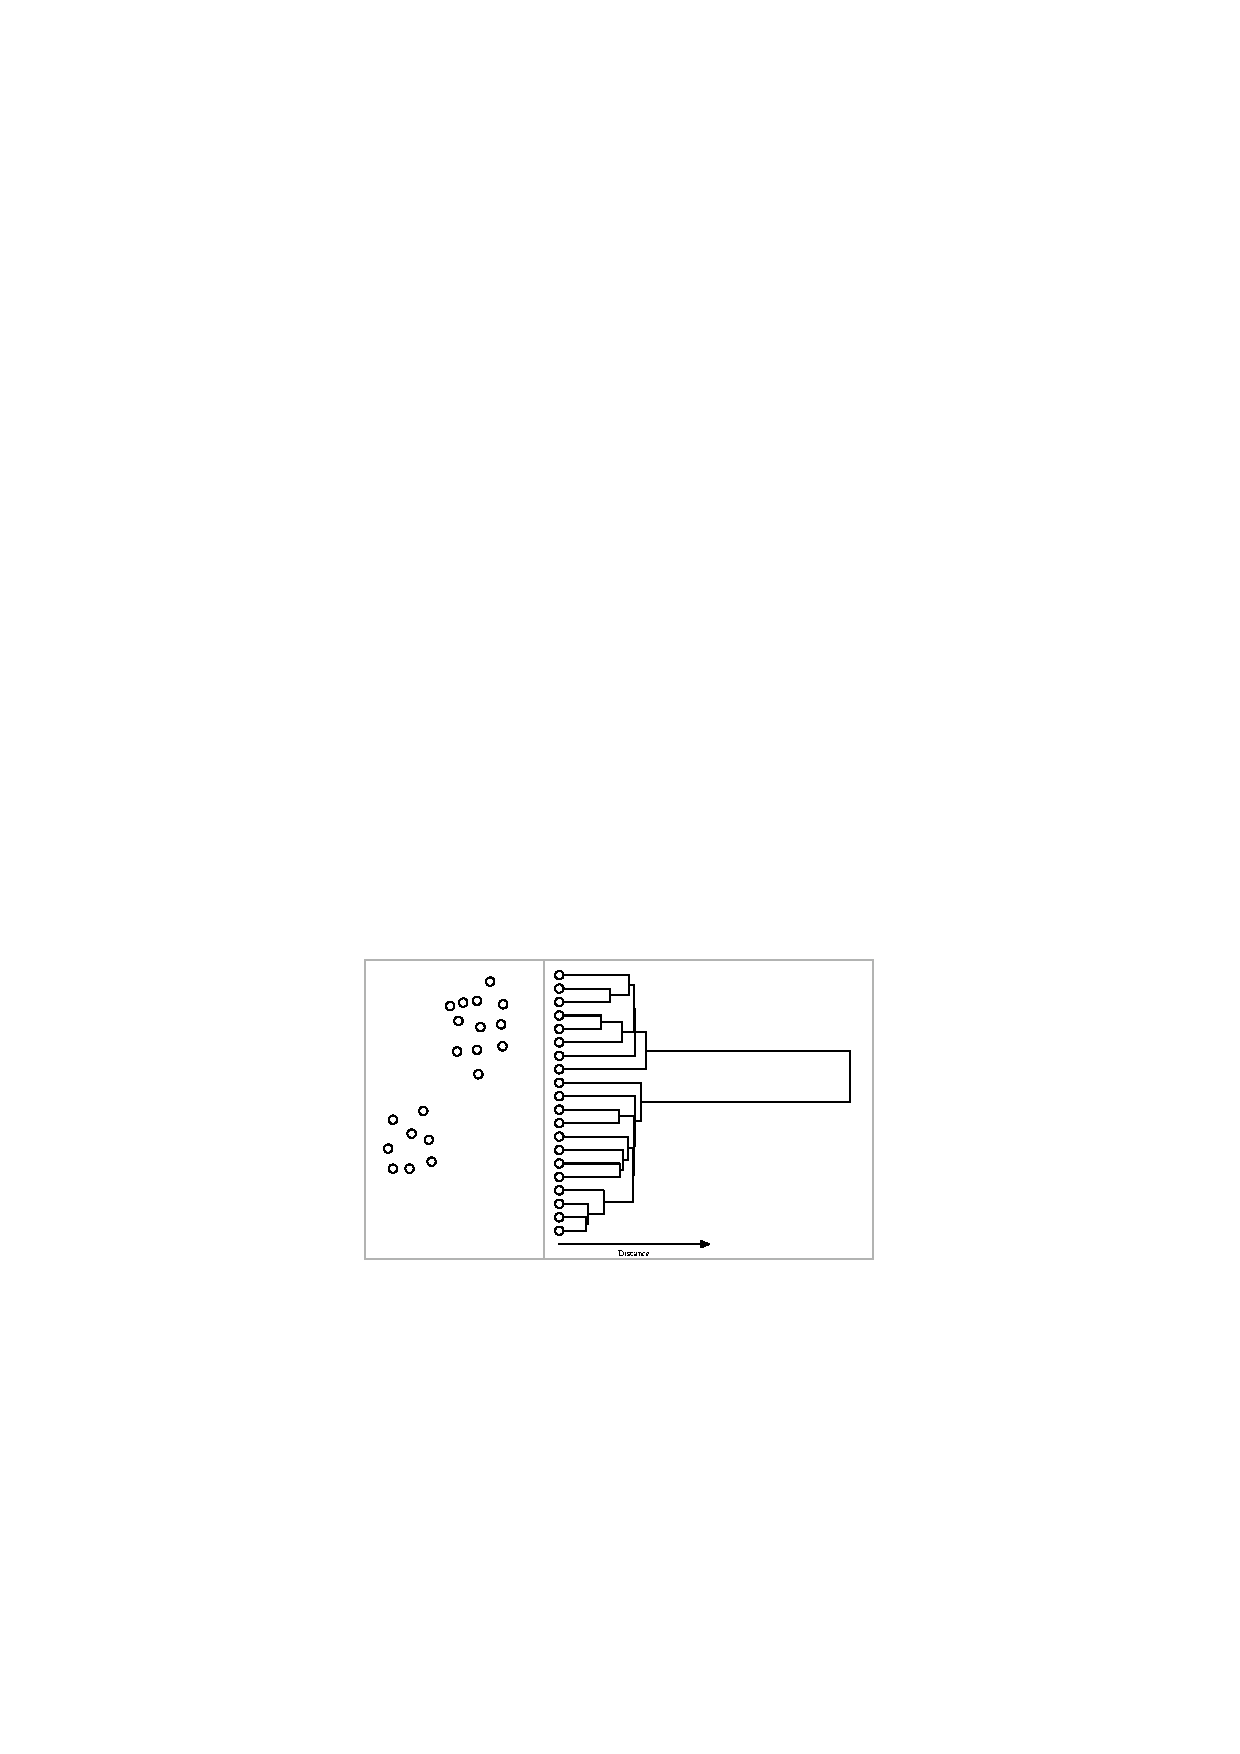
\includegraphics[width=0.9\textwidth]{figures/clustering_hierarchical_dendrogram.pdf}
    \caption{Dendrogram~\cite[p 20]{Meert06clustermaps}.}
    \label{fig:clustering-hierarchical-dendrogram}
  \end{center}
\end{figure}


\subsection{Density-based clustering algorithms: DBSCAN}

Density-based algorithms cluster regions of high density and separate them from regions with lower density. The density-based approach is different to the previously discussed distance-based methods. Those tend to perform well in the detection of spherical-shaped clusters, but discovering arbitrary shapes is a problem. Density-based algorithms overcome this limitation and are also insensitive to noise points, so that outliers get isolated.

\begin{algorithm}[t]
  \While{Point is unclassified}{
    {Find points within region $\epsilon$}\;
    \If{number of points within region $> MinPts$} {
      {Start new cluster with Point}\;
      {Search regions of points in new cluster and expand cluster}\;
    }
  }
  \caption{DBSCAN algorithm~\cite{Meert06clustermaps}}
  \label{alg:dbscan}
\end{algorithm}

\textit{DBSCAN} starts with an unclassified point. Subsequently, the density of the point is calculated by computing all its neighborhood points within a radius $\epsilon$. Based on the density, the algorithm classifies points as \textit{core points}, \textit{border points} or \textit{noise points}:

\begin{itemize}
\item \textit{core points} have a number of points within their neighborhood that exceeds the threshold defined as $MinPts$
\item \textit{border points} don't match the previous criterion but they themselves fall into the neighborhood of another core point
\item \textit{noise points} are outside of any neighborhood and therefore are neither core points nor border points
\end{itemize}

Any core point will be expanded to a cluster in the procedure until every point has been classified~\cite{Varlaro08spatial, Meert06clustermaps}.

The quadratic time complexity of DBSCAN \BigO{n^2} can be optimized by using an indexing structure for the neighborhood queries~\cite{wiki:DBSCAN}:
\[time~complexity = \BigO{n \log{n} }\]

Figure~\ref{fig:clustering-dbscan} illustrates a DBSCAN clustering process.

\begin{figure}[h]
  \begin{center}
    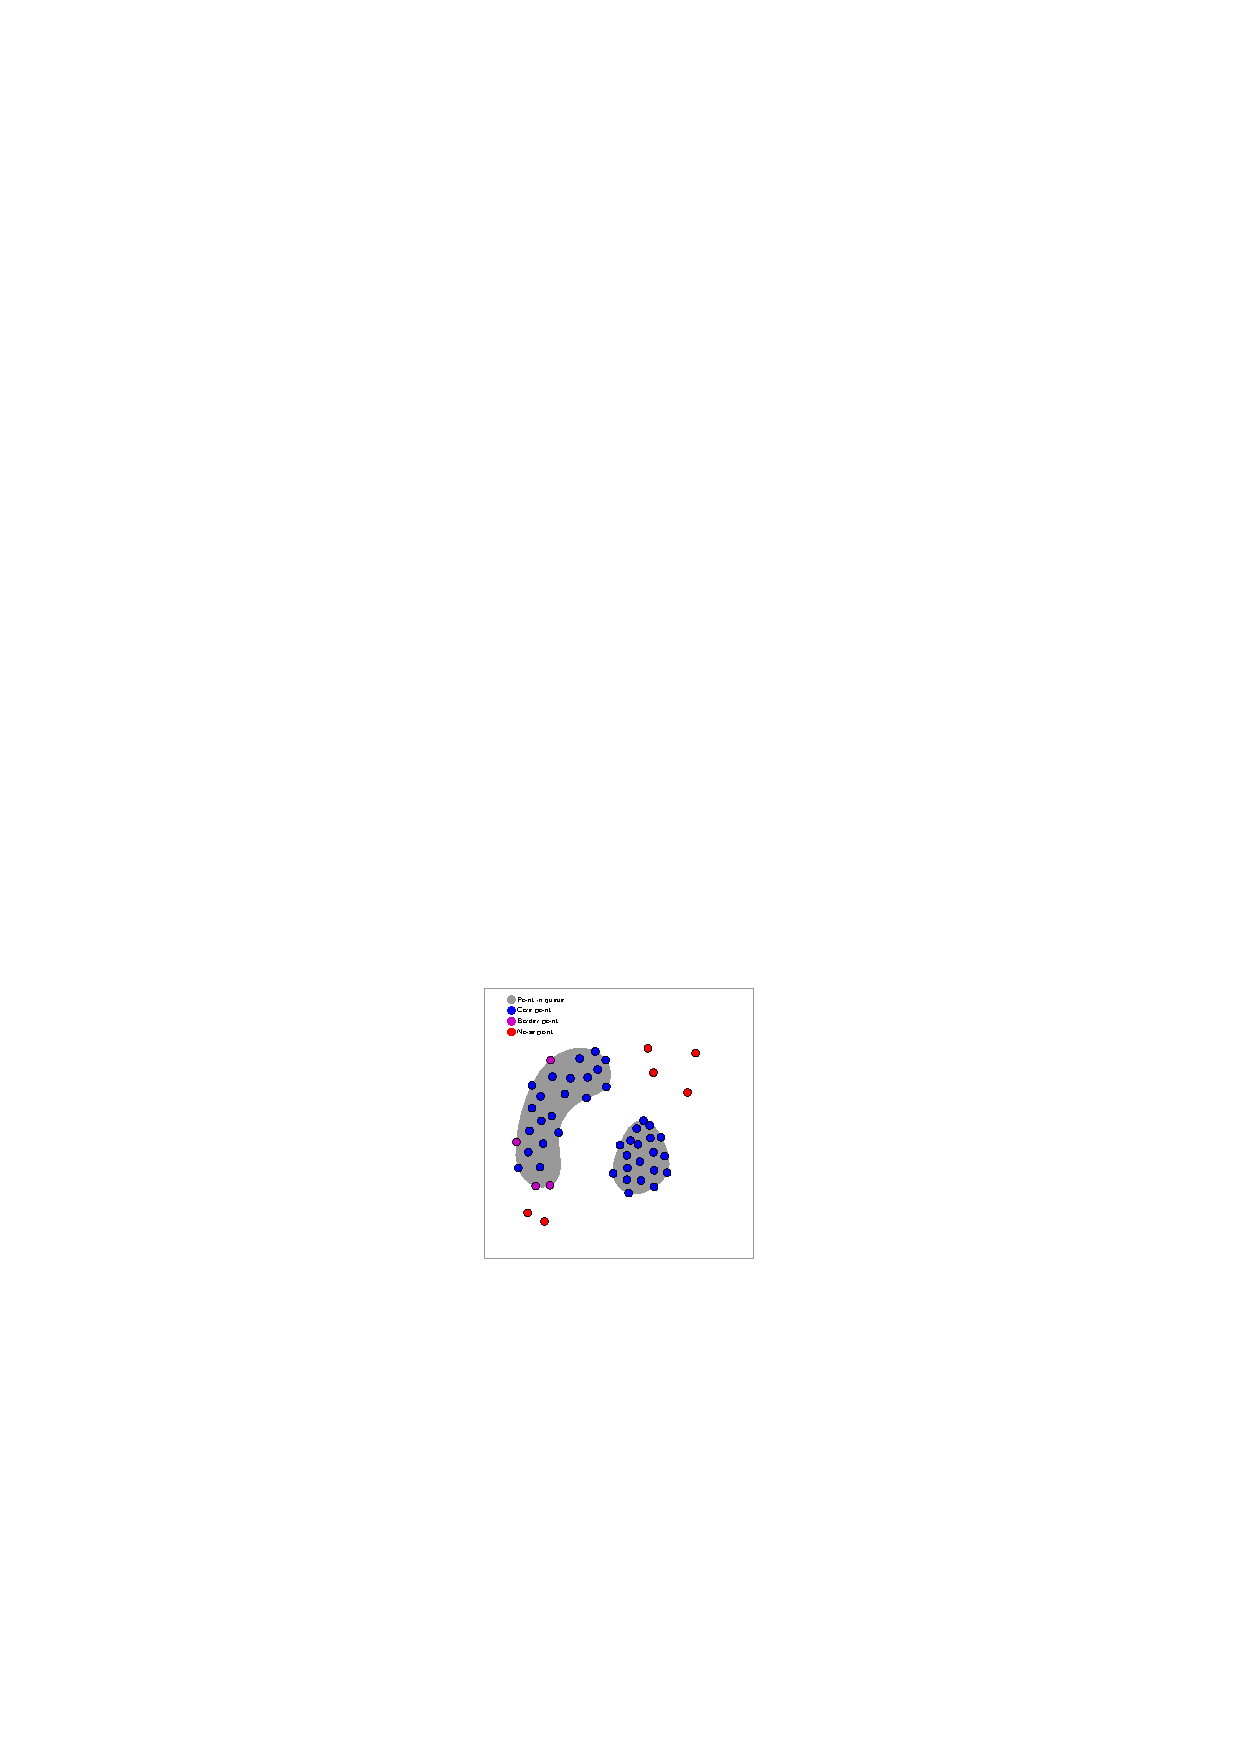
\includegraphics[width=0.55\textwidth]{figures/clustering_dbscan.pdf}
    \caption{DBSCAN algorithm~\cite[p 26]{Meert06clustermaps}.}
    \label{fig:clustering-dbscan}
  \end{center}
\end{figure}

\subsection{Grid-based algorithms: STING}
\label{chapter:clustering-grid}

The time complexity of the previously discussed algorithms is at least linear to the number of points that have to be clustered. Grid-based algorithms overcome this performance limitation by partitioning data to be clustered in a grid structure. The clustering process is executed on pre clustered cells of the grid structure, which obviously scales better.

The STING algorithm takes such a grid-based approach and divides the data points into a grid of rectangular cells. The cells form a hierarchical structure, so that different levels of grids correspond to different resolutions. Every cell in the grid is sub-divided into a further partitioning one level deeper in the hierarchy. STING therefore precomputes a hierarchical index with various levels of granularity on which the clustering process is later executed. The name-giving property of STING (Statistical INformation Grid) is that each cell contains statistical information which can be used to answer queries. 

The time complexity can be shifted to the computation of the grid which is linear to the points of data $\BigO{n}$. The query processing time is reduced to $\BigO{g}$, where $g$ is the constant of number of cells at the bottom level of the computed hierarchy. As per the construction of the hierarchy, it can be assumed that $g \ll n$~\cite{Varlaro08spatial, Wang97sting}.  

Figure~\ref{fig:clustering-sting} illustrates a hierarchical grid used in the STING clustering process.

\begin{figure}[h]
  \begin{center}
    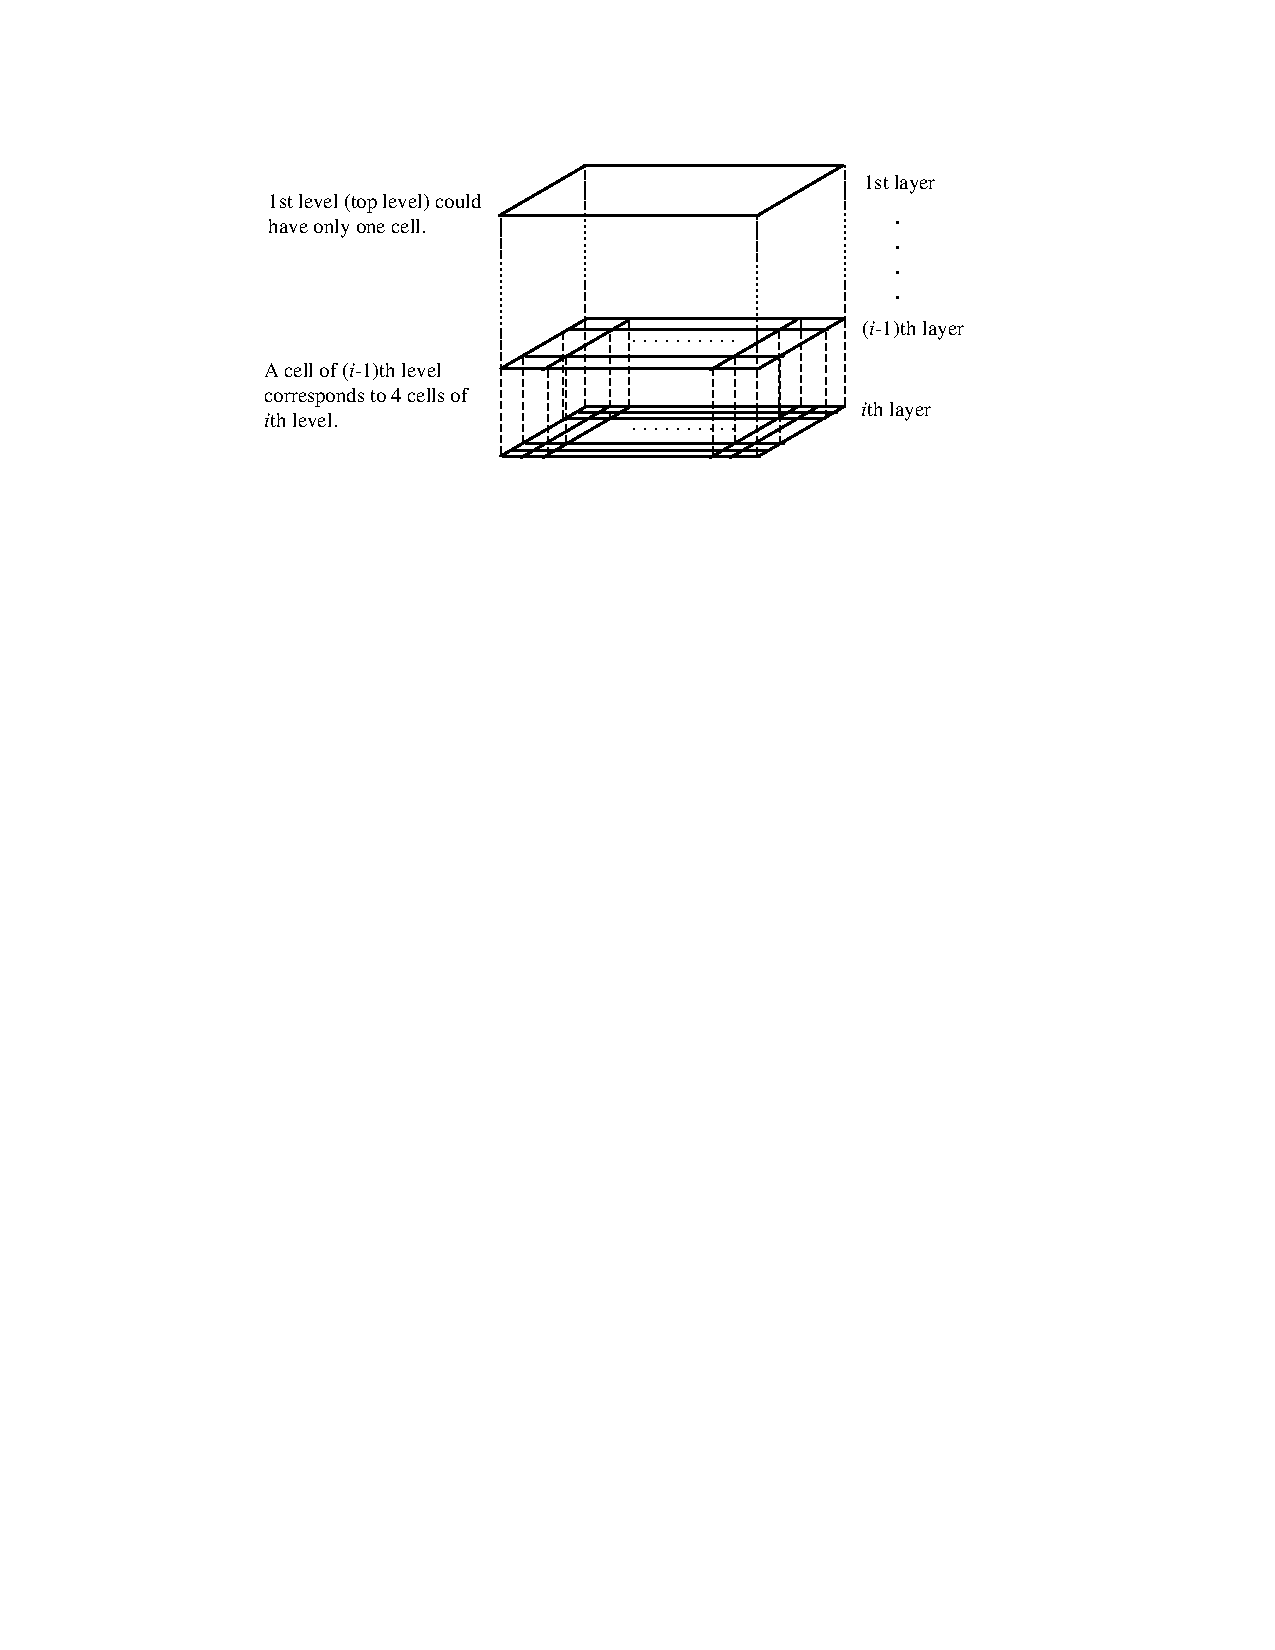
\includegraphics[width=0.9\textwidth]{figures/clustering_sting.pdf}
    \caption{Hierarchical Structure of the STING algorithm~\cite[p 5]{Wang97sting}.}
    \label{fig:clustering-sting}
  \end{center}
\end{figure}




















